\chapter{THE LARGE HADRON COLLIDER AND THE CMS EXPERIMENT} \label{lhc-cms}

\section{Large Hadron Collider}
The Large Hadron Collider is a particle collider near Geneva, Switzerland run by the European Organization for Nuclear Research (CERN). The LHC is the largest and most powerful particle collider ever built, designed to collide protons with a center of mass energy of 14 TeV and a luminosity of $10^{34} {\rm cm^{-2}s^{-1}}$ \cite{LHC}. The luminosity is given by

\begin{equation}
L = \frac{n_{b} f N^{2}_{p} \gamma}{4\pi\epsilon_{n}\beta^{*}}
\end{equation}
where $n_{b}$ is the number of bunches in each ring, f is the frequency for a bunch to circle the ring, ${\rm N_{p}}$ gives the number of protons in a bunch, and ${\rm \gamma}$ is the Lorentz factor. ${\rm \epsilon_{n}}$ is the normalized transverse emittance, a measure of the spread of the beam in momentum and position space. ${\rm \beta^{*}}$ measures the focus of the beam at the interaction point. ${\rm \epsilon_{n}\beta^{*}}$ represents the transverse area at the point of interaction.

The collider itself is 26.7 km in circumference 45-170 m underground. 8.3 T supercooled superconducting magnets operating at 2 K steer the high energy proton beams. In order to save money the LHC not only reuses the tunnels of a previous collider, the Large Electron Positron Collider (LEP), but also reuses older accelerators which were state of the art at their time. These older accelerators ramp up the energy of the protons and inject them into the LHC. All of this together makes up the CERN accelerator complex.

\begin{figure}[h!]
  \centering
  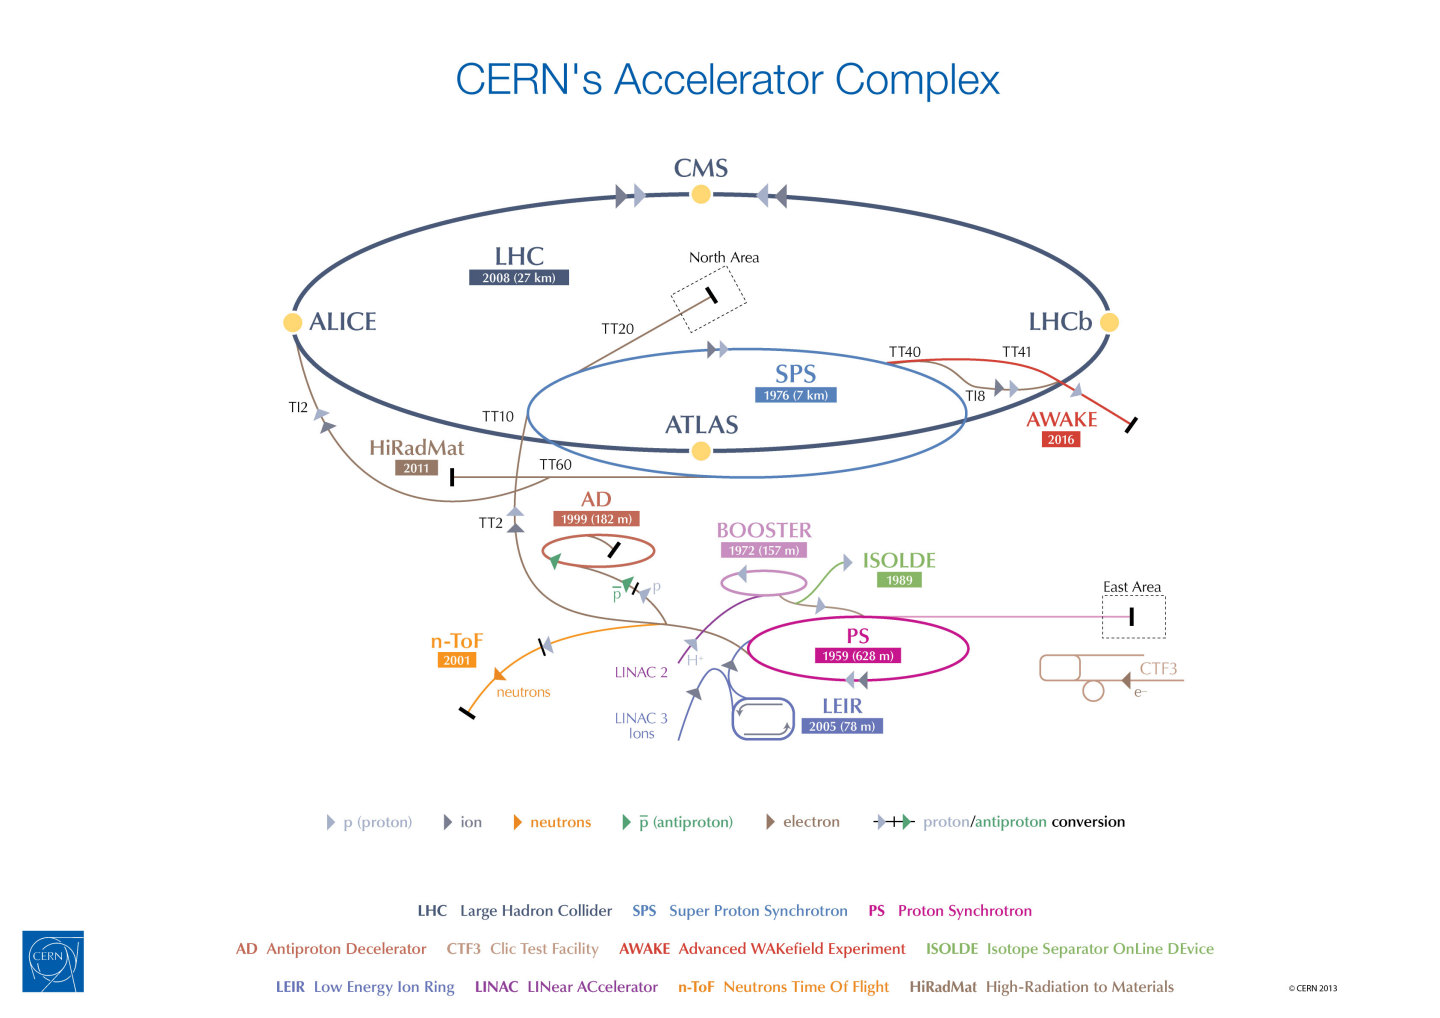
\includegraphics[width=6in]{../images/cern_accel_complex.jpg}
  \caption
   {The CERN Accelerator Complex \cite{cernaccelcomplex}}
  \label{fig:cernaccel}
\end{figure}

Protons start from the ion source and proceed to LINAC2 where they are accelerated to 50 MeV. These protons are then injected into the Proton Synchrotron Booster (PSB) accelerating the protons to 1.4 GeV. From here the protons are injected into the Proton Synchrotron (PS) and accelerate to 25 GeV. The PS then injects the protons into the Super Proton Synchrotron (SPS) further accelerating them to 450 GeV. Finally the protons are injected into the LHC where they accelerate up to 13 TeV. Once accelerated to the appropriate collision energy, the proton beams are made to collide in the different detectors located around the ring. By colliding protons at large enough energies it is possible to create particles iand probe corners of physics that have never been seen before. The two general purpose detectors at the LHC, ALTAS and CMS, are used to measure signs of new physics like the Higgs boson, dark matter, and extra dimensions.

